\subsection{Geschichte der Compact Disc}
\label{subsec:cdgeschichte}

Die Entwicklung von optischen Datenträgern mit einem laserbasiertem
Auslesesystem begann in den 70er Jahren des 20. Jahrhunderts. 1975 brachte
Philips den ersten optischen Datenträger auf den Markt, die Laservision
Videodisc (siehe \autoref{fig:videodisc}). Sie sollte eine Alternative zum
VHS-Videosystem (siehe \autoref{fig:vhs}) darstellen, war jedoch aufgrund der
geringen Verkaufszahlen nicht erfolgreich.

\begin{figure}[h]
    \begin{center}
        \begin{minipage}[t]{0.3\textwidth}
            \begin{center}
                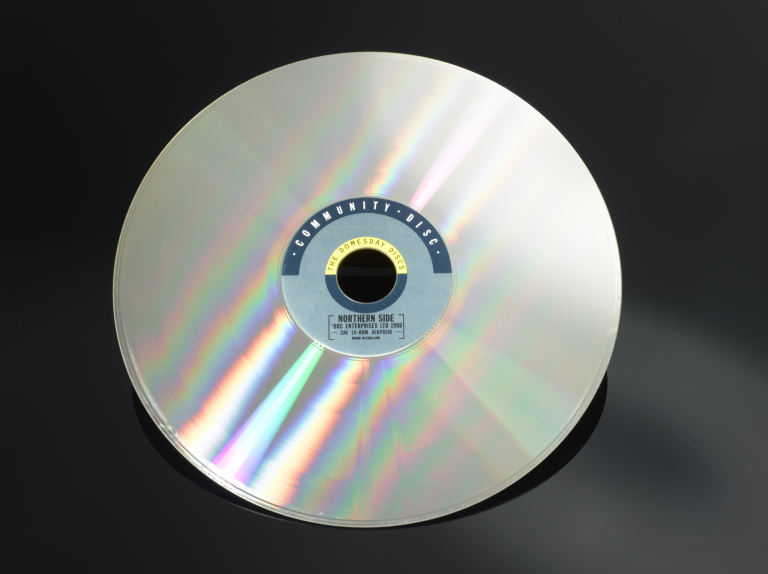
\includegraphics[height=0.1\textheight]{Bilder/Optische_Datentraeger_Die_Compact_Disc/Geschichte/videodisc.png}
                \caption[Laservision Videodisc \newline \url{http://www.sciencemuseum.org.uk/online_science/explore_our_collections/objects/index/smxg-8095649} (zuletzt aufgerufen am 19.09.2015)]{Laservision \newline Videodisc}
                \label{fig:videodisc}
            \end{center}
        \end{minipage}
        \hspace{0.025\textwidth}
        \begin{minipage}[t]{0.3\textwidth}
            \begin{center}
                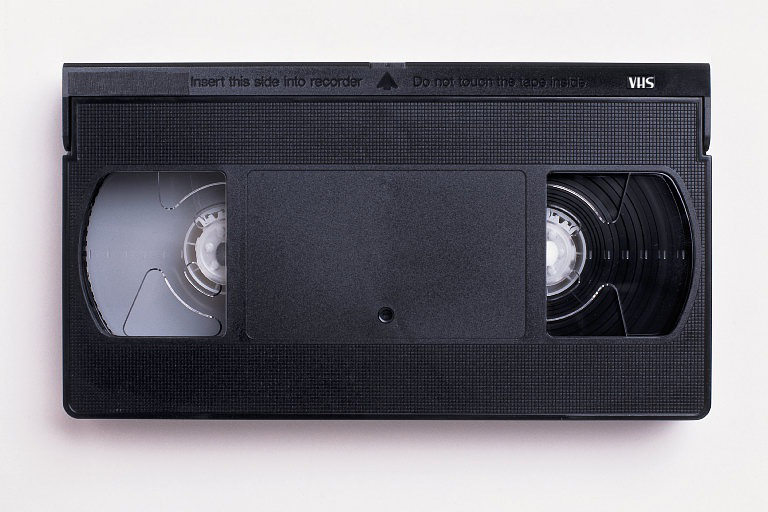
\includegraphics[height=0.1\textheight]{Bilder/Optische_Datentraeger_Die_Compact_Disc/Geschichte/vhs.png}
                \caption[VHS cassette \newline \url{https://upload.wikimedia.org/wikipedia/commons/6/67/VHS-cassette.jpg} (zuletzt aufgerufen am 19.09.2015)]{VHS Cassette}
                \label{fig:vhs}
            \end{center}
        \end{minipage}
    \end{center}
\end{figure}

Auf Basis der Videodisc entwickelte Philips bis 1977 die Compact Disc Digital
Audio mit einem Durchmesser von 11,5 cm und einer Spielzeit von 60 Minuten.

Ab 1979 arbeiteten Philips und Sony dann an einem gemeinsamen CD-Standard mit
einem Durchmesser von 12 cm und einer 75-minütige Spielzeit. Dieser Standard
wird bis heute von allen CD-Herstellern anerkannt. \cite{cds}

Die Schallplattenproduzenten befürchteten rückläufige Verkaufszahlen. Deshalb
scheiterten die Verhandlungen betreffend die Rechte an Musikstücken für CDs.

Zunächst konzentrierten sich Philips und Sony auf klassische Musik, da die
beiden Unternehmen annahme, dass dieser Kundenstamm für eine bessere
Klangqualität mehr Geld auszugeben bereit wäre. %TODO: CHECK

Der CD gelang der Durchbruch während der Salzburger Festspiele im April 1981.
Philips und Sony konnten ein Publikum aus Musikkritikern von dem
Zukunftspotential der CD überzeugen. Die Begeisterung der Kritiker erfasste die
internationale Musikszene und bis März 1982 hatten acht Schallplattenfirmen
Verträge mit Philips und Sony unterschrieben. Die Markteinführung erfolgte am
17. August 1982. \cite{cuz}

Innerhalb weniger verdrängte Jahre die CD die Schallplatte fast komplett vom
Markt. \autoref{fig:umsatzcd} zeigt den Umsatz der deutschen Musikindustrie mit
den jeweiligen Produkten. Der Umsatz mit Vinylschallplatten, 1980 mit ca. 760
Mio. Euro noch das umsatzstärkste Medium, sank bis 1987 erst all­mäh­lich und
dann bis 1992 rapide. Im selben Zeitraum stieg der Umsatz mit CDs massiv an und
erreichte im Jahr 1997 ein Maximum von 2,3 Mrd. Euro. Ab 1997 waren die
Verkaufszahlen rückläufig, da Privatperson selbst CDs
\shorthandoff{"}"brennen"\shorthandon{"} konnten und zunehmend legale und
illegale Angebote im Internet nutzten.

\begin{figure}[h]
    \begin{center}
        \begin{minipage}[t]{\textwidth}
            \begin{center}
                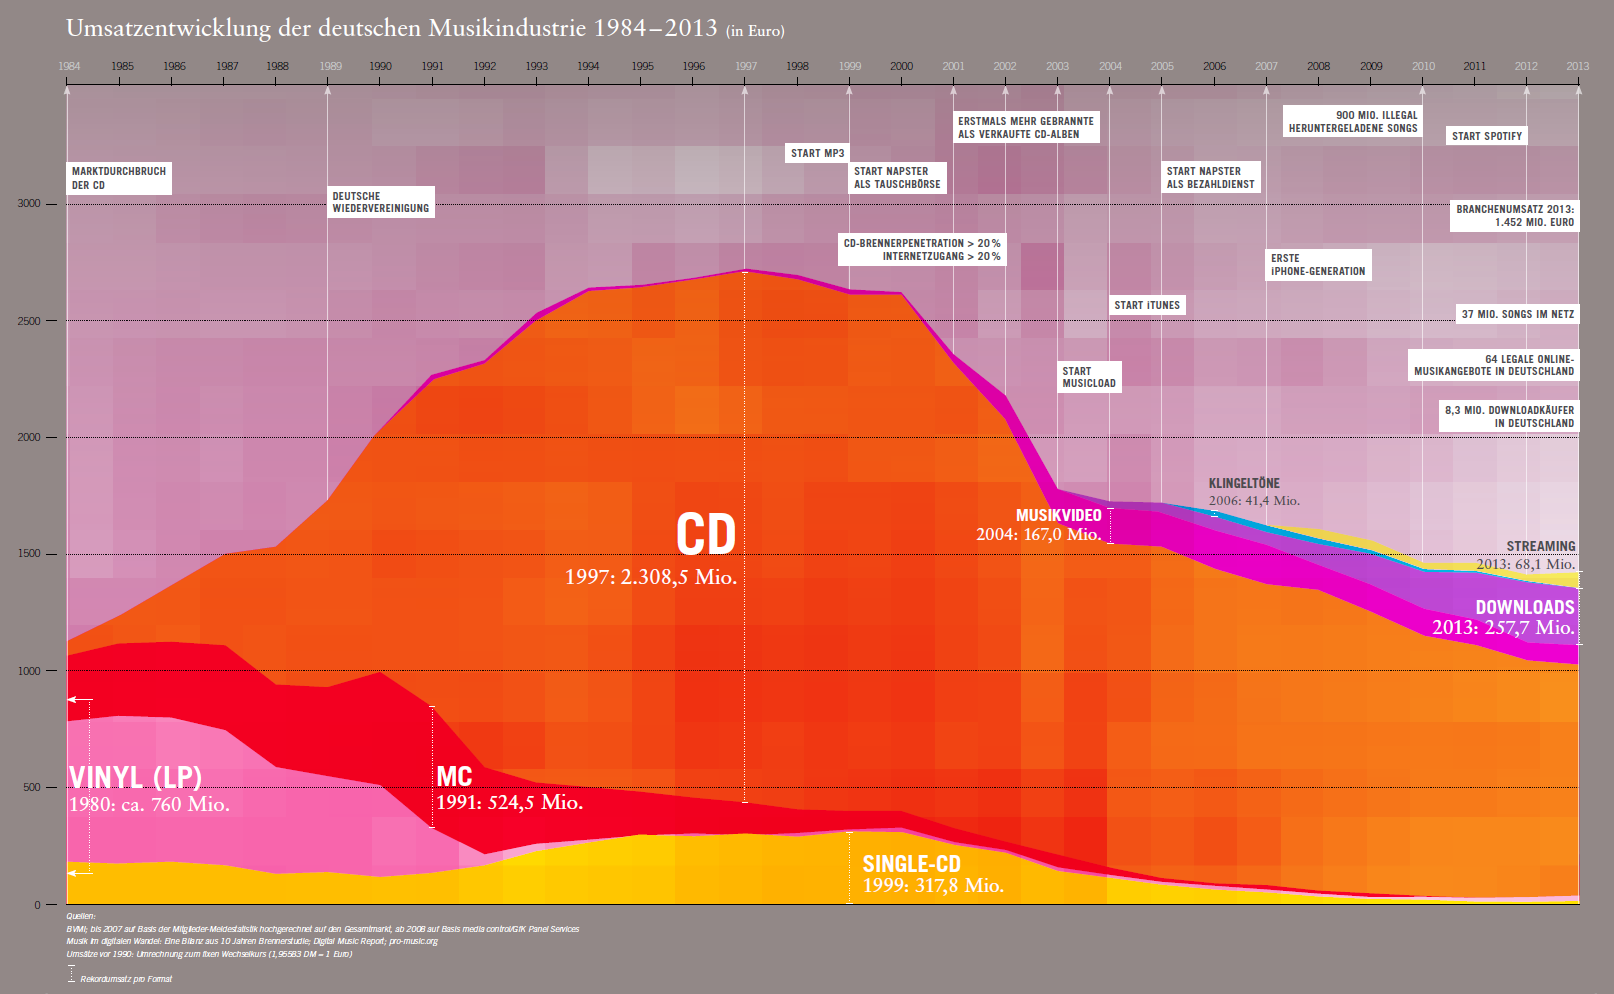
\includegraphics[width=\textwidth]{Bilder/Optische_Datentraeger_Die_Compact_Disc/Geschichte/umsatzcd.png}
                \caption[Umsatzentwicklung der deutschen Musikindustrie \newline \url{http://www.musikindustrie.de/uploads/media/140325\_BVMI\_2013\_Jahrbuch\_ePaper\_V02.pdf} S. 7 (zuletzt aufgerufen am 03.08.2015)]{Umsatzentwicklung der deutschen Musikindustrie}
                \label{fig:umsatzcd}
            \end{center}
        \end{minipage}
    \end{center}
\end{figure}
